\chapter{Generalized compressed suffix array}\label{chapter:gcsa}

The compressed suffix arrays discussed so far index either single sequences or collections of sequences. This is not a fundamental limitation, however. In this chapter, based on Paper~IV, we generalize the compressed suffix arrays to handle a certain class finite automata. This class of automata can recognize all finite languages and some infinite languages as well.

Backward searching using BWT is based on the following property: text positions containing character $c$ are sorted in the same order as text positions preceded by character $c$. If we consider the sequence a finite automaton, we could say that nodes labeled with character $c$ are sorted in the same order as those nodes with a predecessor labeled with character $c$. To use this idea to index finite automata, we need to solve two problems: handling nodes with multiple predecessors or successors (Section~\ref{sect:gcsa}), and constructing an automaton that can be sorted in the desired way (Section~\ref{sect:gcsa construction}).

In the general case, the sorted automaton can be exponentially larger than the minimal deterministic automaton recognizing the same language. However, if only a small fraction of the nodes of the minimal automaton have multiple successors, most of the nodes can be sorted by the label of the unique path of length $k$ (for some $k > 0$) starting from the node. For these languages, the sorted automaton is not much larger than the minimal one. An important example of this kind of automata are those arising from a reference sequence and a set of substitutions, insertions, and deletions, or from a multiple alignment of sequences. In the latter case, the automaton will recognize not only the original sequences, but all their plausible recombinations as well.
\newpage


\section{Indexing finite languages}\label{sect:gcsa}

The {\em XBW transform} \cite{Ferragina2009b} is a generalization of the Burrows-Wheeler transform for labeled trees, where leaf nodes and internal nodes are labeled with different alphabets. Each internal node of the tree is represented as a concatenation of the labels of its children. These representations, sorted in lexicographic order according to the path labels from the node to the root, form sequence $\BWT$. The starting position of each internal node in $\BWT$ is marked by an \onebit{} in bit vector $F$, so that the node with lexicographic rank $i$ can be found as $\BWT[\mselect_{1}(F,i), \mselect_{1}(F,i+1) - 1]$.

XBW supports tree navigation with generalizations of functions $LF$ and $\Psi$. In downward functions such as $LF$, the lexicographic ranks returned by the regular versions of the functions are converted into BWT ranges by using \select{} on bit vector $F$, as above. Upward functions such as $\Psi$ work in the opposite way, converting BWT ranges into lexicographic ranks by using \rank{} on bit vector $F$, before calling the regular version of the function.

\paragraph{Generalization for finite automata.}

Bit vector $F$, mapping lexicographic ranks into BWT ranges, allows a single node to have multiple predecessors. We can use a similar idea to allow multiple successors, extending XBW from trees to finite automata. The idea is to use another bit vector $M$ to encode the number of outgoing edges, so that the node with lexicographic rank $i$ has $\mselect_{1}(M,i+1) - \mselect_{1}(M,i)$ outgoing edges.\footnote{This definition of bit vector $M$ makes the generalization simpler than the original definition.} For convenience, we assume that the final node $V_{\abs{V}}$ has a single outgoing edge to the initial node $V_{1}$.

Backward navigation ($LF$) first uses bit vector $F$ to convert lexicographic ranks into a BWT range, then calls the regular version of the function, and finally uses bit vector $M$ to convert the edge range into lexicographic ranks. Forward navigation ($\Psi$) uses bit vectors $M$ and $F$ in the opposite way. See Figure~\ref{fig:gcsa navigation} for pseudocode for basic navigation functions, and below for exact definitions of the functions.

\begin{figure}[t!]\centering
\begin{tabbing}
mm\=mm\=mm\= \kill
{\bf function} $\operatorname{LF}([sp,ep], c)$ \\
\> $[sp, ep] \leftarrow [\mselect_{1}(F,sp), \mselect_{1}(F,ep+1) - 1]$ \\
\> $[sp, ep] \leftarrow [C[c] + \mrank_{c}(\BWT, sp - 1) + 1, C[c] + \mrank_{c}(\BWT, ep)]$ \\
\> $[sp, ep] \leftarrow [\mrank_{1}(M,sp), \mrank_{1}(M,ep)]$ \\
\> {\bf return} $[sp,ep]$ \\
\\
{\bf function} $\Psi(i, j)$ \\
\> $c \leftarrow \mchar(i)$ \\
\> $i \leftarrow \mselect_{1}(M,i) + j - 1$ \\
\> $i \leftarrow \mselect_{c}(\BWT, i - C[c])$ \\
\> $i \leftarrow \mrank_{1}(F,i)$ \\
\> {\bf return} $i$
\end{tabbing}

\caption{Pseudocode for the basic navigation functions $LF$ and $\Psi$.}\label{fig:gcsa navigation}
\end{figure}

\paragraph{Definitions.}

As mentioned in the beginning of the chapter, the automaton must have a certain property in order for functions $LF$ and $\Psi$ to work. We call this property prefix-range-sortedness.

\begin{definition}\label{def:prefix-range-sorted}
Let $A = (V, E)$ be a finite automaton, and let $v \in V$ be a node. Let $rng(v)$ be the smallest (open, semiopen, or closed) lexicographic range containing all suffixes that can be recognized from node $v$. Node $v$ is {\em prefix-range-sorted}, if no suffix $S \in rng(v)$ is recognized from any other node $v' \ne v$. Automaton $A$ is prefix-range-sorted, if all nodes are prefix-range-sorted.
\end{definition}

In the following, we use a stronger definition to simplify the discussion. The results for prefix-sorted automata generalize for prefix-range-sorted automata as well.

\begin{definition}\label{def:prefix-sorted}
Let $A$ be a finite automaton, and let $v \in V$ be a node. Node $v$ is {\em prefix-sorted} by prefix $p(v)$, if the labels of all paths from $v$ to $v_{\abs{V}}$ share a common prefix $p(v)$, and no path from any other node $u \ne v$ to $v_{\abs{V}}$ has $p(v)$ as a prefix of its label. Automaton $A$ is prefix-sorted, if all nodes are prefix-sorted.
\end{definition}

We can use the prefixes $p(v)$ to sort the nodes of a prefix-sorted automaton in lexicographic order. If we do so, then we have also sorted the outgoing edges $(u,v)$ using sequences $\ell(u) p(v)$ as sort keys, and the edge encoded by bit $M[i]$ has lexicographic rank $i$. This is the key for functions $LF$ and $\Psi$ to work properly. For any given character $c$, all outgoing edges from nodes with label $c$ are lexicographically adjacent, and they are sorted by prefix $p(v)$ of the destination node. Similarly, all occurrences of character $c$ in $\BWT$ encode an incoming edge from a node with label $c$, and these edges are also sorted by prefix $p(v)$ of the destination node. Hence the incoming edge labeled by the $j$th occurrence of character $c$ is the same edge as the outgoing edge of rank $C[c] + j$, and the other way around. Note that $C[c]$ stores the number of occurrences of characters smaller than $c$ in $\BWT$, not the number of nodes with label smaller than $c$.

\paragraph{Operations.}

We define the basic navigation functions in the following way.
\begin{itemize}
\item $LF([sp,ep], c)$ is the lexicographic range of nodes with label $c$ that have a successor in the lexicographic range $[sp,ep]$. This is essentially a step of backward searching with character $c$.
\item $\Psi(i, j)$ is the lexicographic rank of the $j$th successor of the node with lexicographic rank $i$.
\item $\mchar(i)$ is the label of the node with lexicographic rank $i$.
\end{itemize}

These operations can be used to support the following generalization of suffix array functionality (see Definition~\ref{def:suffix array}).
\begin{itemize}
\item \find($P$) returns the lexicographic range $[sp, ep]$ of nodes recognizing any suffix that has pattern $P$ as its prefix.
\item \locate($i$) returns a numerical value corresponding to the node with lexicographic rank $i$.
\item \extract($i, \Path$) returns the label of path $\Path$ starting from the node with lexicographic rank $i$.
\end{itemize}

We can support \find{} by replacing the first two lines of the loop body in Figure~\ref{fig:backward searching} with function $LF$ from Figure~\ref{fig:gcsa navigation}.

For \locate, we assume that there is a (not necessarily unique) numerical value $id(v)$ attached to each node $v \in V$. Examples of these values include node ids (so that $id(v_{i}) = i$) and positions in a multiple alignment. To avoid excessive sampling of node values, $id(v)$ should be $id(u) + 1$ whenever $(u,v)$ is the only outgoing edge from $u$ and the only incoming edge to $v$.

We sample $id(u)$, if there are multiple outgoing edges from node $u$, or if $id(v) \ne id(u) + 1$ for the only outgoing edge $(u, v)$. We also sample one out of $d$ node values, given sample rate $d > 0$, on paths of at least $d$ nodes without any samples. The sampled values are stored in the same order as the nodes, and their positions are marked in bit vector $B_{s}$.

As we have sampled all nodes with multiple successors, we can use the \locate{} algorithm of the CSA family directly with our new function $\Psi$. To retrieve $id(u)$ for node $u$ of lexicographic rank $i$, we first check if $B_{s}[i] = 1$, and return sample $rank_{1}(B_{s}, i)$, if this is the case. Otherwise we follow the only outgoing edge $(u,v)$ by using function $\Psi$, and continue from node $v$. When we find a sampled node $w$, we return $id(w) - k$, where $k$ is the number of steps taken by using $\Psi$.

In \extract, we assume that the description of path $\Path$ allows us to determine in constant time, which outgoing edge we should take, and have we already finished the path. With such description, we can use function $\Psi$ to move forward on the path, and function $\mchar(\cdot)$ to read the next character of the path label. The algorithm is similar to the \extract{} algorithm of the CSA family, with the exception that we already know the lexicographic rank of the initial node. This is because we might be using a node value scheme that does not allow mapping node values to lexicographic ranks.

We call a compressed self-index based on this generalization of the XBW transform a \emph{generalized compressed suffix array (GCSA)}. As each step of $LF$ and $\Psi$ requires both \rank{} and \select, we get the following generalization of Theorem~\ref{theorem:csa}.

\begin{theorem}\label{theorem:gcsa}
Let \rank\ and \select\ on binary sequences take $t_{R}$ and $t_{S}$ time, respectively. Then a generalized compressed suffix array with sample rate $d$ supports \find$(P)$ in $O(\abs{P} \cdot (t_{R} + t_{S}))$ time, \locate\ in $O(d \cdot (t_{R} + t_{S}))$ time, and \extract$(i, \Path)$ in $O(\abs{\Path}(t_{R} + t_{S}))$ time.
\end{theorem}

\paragraph{A better encoding.}

Recall that the size bound of RLCSA (Theorem~\ref{theorem:rlcsa}) is worse than for plain run-length encoding of the BWT (Section~\ref{sect:compression}). This is because RLCSA has to encode each character of $\BWT$ with either a \zerobit{} or an \onebit{} in every bit vector $B_{c}$, while the run-length encoding encodes each character only once. In GCSA, we can use this redundancy for our advantage.

As a prefix-range sorted automaton is reverse deterministic, each node can have at most one predecessor with a certain label. Hence the section of $\BWT$ corresponding to a node can have at most one occurrence of each character, meaning that we can put all these predecessor labels into the same position in bit vectors $B_{c}$. As the bit $B_{c}[i]$ now determines, whether the node with lexicographic rank $i$ has a predecessor with label $c$, we no longer have to use bit vector $F$ to map between lexicographic ranks and BWT ranges. This is a major speedup in practice, as we get rid of one third of bit vector operations.


\section{Construction algorithm}\label{sect:gcsa construction}

A straightforward way of constructing a prefix-sorted automaton from a finite automaton recognizing a finite language is via a prefix-doubling algorithm (see Section~\ref{sect:construction implementation}). The algorithm consists mostly of sorting, scanning, and database joins. Hence it can be efficiently implemented in parallel, distributed, and external memory settings.

\begin{theorem}
Assume we have a length $n$ multiple alignment of $r$ sequences over alphabet of size $\sigma$. We can build a prefix-range-sorted automaton recognizing all paths through the alignment in $O(nr + \abs{V'} \log n + \abs{E'})$ time and $O(nr \log \sigma + \abs{V'} \log \abs{V'} + \abs{E'} \log \abs{E'})$ bits of space, where $V'$ and $E'$ are the largest intermediate sets of nodes and edges, respectively.
\end{theorem}

\begin{proof}
From Lemmas \ref{lemma:automaton construction}, \ref{lemma:node construction}, and \ref{lemma:edge construction} below.
\end{proof}

The sizes of the largest intermediate sets of nodes and edges are analyzed in a restricted model in Section~\ref{sect:gcsa analysis}. An example of construction can be seen in Figures~\ref{fig:automaton} and \ref{fig:prefix-sorted automaton} and Table~\ref{table:gcsa example}.

\begin{figure}
\centerline{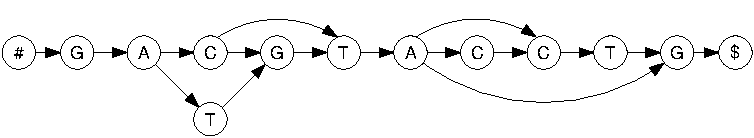
\includegraphics{figures/automaton.pdf}}
\caption{A reverse deterministic automaton corresponding to the first 10 positions of the multiple alignment in Figure~\ref{fig:multiple alignment}.} 
\label{fig:automaton}
\end{figure}

\begin{figure}
\centerline{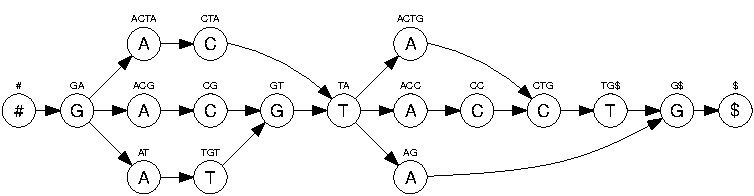
\includegraphics{figures/sorted.pdf}}
\caption{A prefix-sorted automaton built for the automaton in Figure~\ref{fig:automaton}. The strings above nodes are prefixes $p(v)$.} 
\label{fig:prefix-sorted automaton}
\end{figure}

\begin{table}
\centering
\renewcommand{\tabcolsep}{.05cm}
\texttt{
\begin{tabular}{cccccccccccccccccccc}
\hline\noalign{\smallskip}
       & & \$  & ACC & ACG & ACTA & ACTG & AG & AT & CC & CG & CTA & CTG & G\$ & GA   & GT & TA  & TG\$ & TGT & \# \\
\noalign{\smallskip}
\hline
\noalign{\smallskip}
$\BWT$ & & G & T & G & G & T & T & G & A  & A  & A & AC & AT & \#  & CT & CG  & C & A & \$ \\
$M$    & & 1 & 1 & 1 & 1 & 1 & 1 & 1 & 1  & 1  & 1 & 1  & 1  & 100 & 1  & 100 & 1 & 1 & 1  \\
\noalign{\smallskip}
\hline
\end{tabular}}

\caption{GCSA for the automaton in Figure~\ref{fig:prefix-sorted automaton}. Nodes are identified by prefixes $p(v)$.} 
\label{table:gcsa example}
\end{table}

\paragraph{Building a reverse deterministic automaton.}

With the following algorithm, we can build a reverse deterministic automaton that recognizes all paths through a multiple alignment of sequences. The same approach, when used with a reference sequence and a set of edit operations, is essentially a variant of the textbook algorithm for determinizing finite automata.

In the following, we assume that the alignment consists of sequences $S_{1}, \dotsc, S_{r}$ of length $n$, possibly containing gap characters $-$. Sequences $S_{i}$ and $S_{i'}$ are considered to be equivalent at position $j$, if $S_{i}[j] = S_{i'}[j] \ne -$. We can allow edit operations longer than one character by using a context to determine the equivalence of two positions. With context length $k \ge 0$, sequences $S_{i}$ and $S_{i'}$ are equivalent at position $j$, if $S_{i}[j] = S_{i'}[j] \ne -$ and the next $k$ non-gap characters in the sequences are also equal.

The algorithm works in one pass from right to left. Assume that we have already processed positions $j+1$ to $n$ and created the corresponding part of the automaton. For each sequence $S_{i}$ with a non-gap character in column $j$, we first create a temporary node $v_{i,j}$ and an edge from $v_{i,j}$ to the node corresponding to the next non-gap character in sequence $S_{i}$. Next, we merge the temporary nodes for those sequences that are equivalent at position $j$.

Finally, we find the preceding non-gap characters for all sequences with a non-gap character at position $j$. Assume that two or more sequences that are equivalent at position $j$ have $c$ as the preceding non-gap character. If these characters $c$ occur at different positions, we move them all to the rightmost of these positions. This way, the node $v_{i,j}$ corresponding to the equivalent sequences will only have one predecessor with label $c$.

\begin{lemma}\label{lemma:automaton construction}
Let $n$ be the length of the multiple alignment, $r$ the number of sequences, and $\sigma$ the size of the alphabet. Building a reverse deterministic automaton takes $O(nr)$ time and requires $O(nr \log \sigma + \abs{E} \log \abs{E})$ bits of space, where $E$ is the set of edges of the automaton.
\end{lemma}

Note that each position can be processed in $O(r)$ amortized time, regardless of context length, by keeping the suffixes $S_{i}[j]$ in sorted order and maintaining the lengths of the longest common prefixes of lexicographically adjacent suffixes.

\paragraph{Creating a prefix-sorted automaton.}

\begin{definition}
Let $A$ be a finite automaton recognizing a finite language, and let $k > 0$ be an integer. Automaton $A$ is {\em $k$\nobreakdash-sorted} if, for every node $v$, the labels of all paths from $v$ to $v_{\abs{V}}$ share a common prefix $p(v, k)$ of length $k$, or if node $v$ is prefix-sorted by prefix $p(v, k)$ of length at most $k$.
\end{definition}

Every automaton is $1$\nobreakdash-sorted. Automaton $A$ is prefix-sorted if and only if it is $n$\nobreakdash-sorted, where $n$ is the length of the longest string in $L(A)$.

Starting from a reverse deterministic automaton $A = A_{0}$, we create the nodes of automata $A_{i} = (V_{i}, E_{i})$ for $i = 1, 2, \dotsc$ that are $2^{i}$\nobreakdash-sorted, until we get an automaton that is prefix-sorted. For every node $v \in V_{i}$, let $P(v)$ be the path of $A$ corresponding to prefix $p(v, 2^{i})$. We store the first and the last nodes of this path as $\from(v)$ and $to(v)$, and set $rank(v)$ to be the lexicographic rank of prefix $p(v, 2^{i})$ among all distinct prefixes $p(u, 2^{i})$ of nodes $u \in V_{i}$. If node $v$ has unique $rank(v)$ value, then it is prefix-sorted.

The basic step of the algorithm is the {\em doubling} step from $A_{i}$ to $A_{i+1}$. If node $u \in V_{i}$ is prefix-sorted, we {\em duplicate} it as $w \in V_{i+1}$, and set $rank(w) = (rank(u), 0)$. Otherwise we create a {\em joined} node $uv \in V_{i+1}$ for every node $v \in V_{i}$ such that $P(uv) = P(u)P(v)$ is a path in $A$, and set $\ell(uv) = \ell(u)$ and $rank(uv) = (rank(u), rank(v))$. As path $P(uv)$ exists if and only if there is an edge $(to(u), \from(v)) \in E_{0}$, this essentially requires two database joins.\footnote{Juha Kärkkäinen noted that one join is enough, if we replace $to(u)$ with the destination nodes $w$ for all edges $(to(u), w) \in E_{0}$.} When the nodes of $A_{i+1}$ have been created, we sort them by their ranks, and replace the pairs of integers with integer ranks.

The doubling step is followed by the {\em pruning} step, where we merge equivalent nodes. The nodes in $V_{i+1}$ are sorted by their $rank(\cdot)$ values. If all nodes sharing a certain $rank(\cdot)$ value also share their $\from(\cdot)$ node, these nodes are equivalent, and can be merged. Merging makes the resulting node prefix-sorted.

\begin{lemma}\label{lemma:node construction}
Prefix-doubling algorithm creates the nodes of a prefix-sorted automaton equivalent to $A$ in $O(\abs{V'} \log n)$ time and $O(\abs{V'} \log \abs{V'})$ bits of space in addition to automaton $A$, where $V'$ is the largest set of nodes during construction, and $n$ is the length of the longest string in $L(A)$.
\end{lemma}

The lemma assumes using a linear-time integer sorting algorithm.

\paragraph{Creating the edges.}

Let $A = (V, E)$ be a reverse deterministic automaton recognizing a finite language, and let $W$ be the set of nodes of an equivalent prefix-sorted automaton. To create the edges, we first merge nodes with adjacent $rank(\cdot)$ values, if they share their $\from(\cdot)$ node. The resulting set $V'$ is the set of nodes of a prefix-range-sorted automaton $A' = (V', E')$ equivalent to automaton $A$. The set of edges $E'$ can be constructed efficiently from automaton $A$ and the set of nodes $V'$.

The key to edge construction is that for each node $v \in V'$, the set of $\from(u)$ nodes for the predecessors $u$ of node $v$ is the same as the set of predecessors of node $\from(v)$. With automaton $A$ and the set of nodes $V'$, we can output the edges $(u,v) \in E'$ initially as pairs $(\from(u), v)$, sorted by $(\ell(\from(u)), rank(v))$. Note that this is the same order as sorting the edges by $rank(u)$.

We can map nodes $\from(u)$ to nodes $u$ by scanning the sorted lists of nodes and edges. As every node has at least one outgoing edge, and no adjacent nodes share their $\from(\cdot)$ value, all adjacent edges with the same $\from(\cdot)$ values start from the current node. When the $\from(\cdot)$ value changes in the list of edges, we advance to the next node.

\begin{lemma}\label{lemma:edge construction}
Creating the edges of prefix-range-sorted automaton $A'$ takes $O(\abs{W} + \abs{E'})$ time and requires $O(\abs{W} \log \abs{W} + \abs{E'} \log \abs{E'})$ bits of space, where $W$ is the set of nodes of an equivalent prefix-sorted automaton.
\end{lemma}


\section{Analysis}\label{sect:gcsa analysis}

\paragraph{Languages recognized by prefix-range-sorted automata.}

As shown in Section~\ref{sect:gcsa construction}, every finite language can be recognized by a prefix-range-sorted automaton. There are also some infinite languages that can be recognized by such automaton. For example, consider the regular language $\set{ \# x \$ \mid x \in \set{a, b}^{\ast}}$. The minimal automaton recognizing this language is prefix-range-sorted, as each node has a distinct label.

Not all regular languages have prefix-range-sorted automata, however. Consider, for example, the language $L = \set{ \# x \$ \mid x \in \set{a, b}^{\ast} \cup \set{a, c}^{\ast}}$. Assume that there is a prefix-range-sorted automaton that recognizes the language. Suffixes $B_{n} = a^{n} b \$$ and $C_{n} = a^{n} c \$$ must be recognized from different nodes, as $bB_{n}$ is a suffix of language $L$, while $bC_{n}$ is not. Because $B_{n+1} < C_{n+1} < B_{n}$, suffixes $B_{n}$ and $B_{n+1}$ must also be recognized from different nodes. As the automaton must have an infinite number of nodes, it cannot be a finite automaton.

\paragraph{Size of the automaton.}

We analyze the size of the automata created by the doubling algorithm in the following model. 
Let $S[1,n]$ be a reference sequence, and let $p$ be the mutation rate. For each 
position $i = 1, \dots, n$, the initial automaton $A$ has a node $u_{i}$ with 
label $\ell(u_{i}) = S[i]$, randomly chosen from alphabet $\Sigma$. With 
probability $p$, there is also another node $w_{i}$ with a random label 
$\ell(w_{i}) \in \Sigma \setminus \set{S[i]}$. The automaton has edges from all nodes at position $i$ to all nodes at position $i+1$.

\begin{definition}
Let $k > 0$ be an integer. A {\em $k$-path} in an automaton is a path of length $k$, or a shorter path ending at the final node.
\end{definition}

Let $k > 0$ be an integer. For any position $i$, let $X_{i,k}$ be the number $k$-paths starting from position $i$. If there are $j$ mutated positions covered by these paths, then $X_{i,k} = 2^{j}$, and each of the paths has a different label. The number of mutations is binomially distributed, with path length and mutation probability as the parameters. From the moment-generating function for binomial distribution, we get
\begin{equation}\label{eq:expectation}
\Exp{X_{i,k}} = \sum_{j=0}^{k} \Pr(X_{i,k} = 2^{j}) 2^{j} \le (1+p)^{k}.
\end{equation}
For positions $i = 1, \dots, n - k + 1$, this is an equality.

Let $A_{h}$ be the $2^{h}$-sorted automaton created by the prefix-doubling algorithm. By summing Equation~\ref{eq:expectation} for all positions in the reference sequence, and including the initial and the final nodes, we get $N(2^{h}) = n(1+p)^{2^{h}} + 2$ as an upper bound for the expected number of nodes in $A_{h}$. As the expected number of predecessors for any node at position $i > 1$ is $(1+p)$, we get $N(2^{h})(1+p)$ as an upper bound for the expected number of edges.

Consider the expectation $\Exp{X_{i,k} X_{i',k}}$ for a pair of text positions $i < i'$. If $i' \ge i + k$, then the random variables are independent, and the expectation becomes
\begin{equation}\label{eq:independent}
\Exp{X_{i,k} X_{i',k}} = \Exp{X_{i,k}} \Exp{X_{i',k}} \le (1+p)^{2k}.
\end{equation}
Otherwise assume that the paths starting from positions $i$ and $i'$ overlap in $k' < k$ positions. Then the expectation is a product of the expectations of three independent random variables $X_{i,k-k'}$, $X_{i',k'}^{2}$, and $X_{i'+k',k-k'}$. By using the moment-generating function, we get
\begin{equation}\label{eq:dependent}
\Exp{X_{i,k} X_{i',k}}  \le (1+p)^{2(k-k')} (1+3p)^{k'} \le (1+p)^{3k}.
\end{equation}

\begin{definition}
A pair of nodes of automaton $A_{h}$ {\em collides}, if the corresponding $2^{h}$-paths have identical labels.
\end{definition}

Automaton $A_{h}$ is prefix-sorted, if it has no colliding pairs. Two nodes can collide only, if the $2^{h}$-paths are of length $2^{h}$ and start from different positions in the reference sequence. By Equations \ref{eq:independent} and \ref{eq:dependent}, the expected number of colliding pairs is at most
\begin{equation}\label{eq:node bound}
\sum_{i < i'} \Exp{X_{i,2^{h}} X_{i',2^{h}} / \sigma^{2^{h}}} \le  n^{2} (1+p)^{3 \cdot 2^{h}} / \sigma^{2^{h}}.
\end{equation}

\begin{lemma}\label{lemma:expected number of nodes}
Let $n$ be the length of the reference sequence, $\sigma$ the size of the alphabet, and $p < \sigma^{1/3} - 1$ the mutation rate. For any $\varepsilon > 0$, the largest automaton created by the prefix-doubling algorithm has at most $n(1+p)^{k} + 2$ nodes with probability $1-\varepsilon$, where $k = 2 \log_{\sigma} \frac{n^{2}}{\varepsilon} / (1 - 3 \log_{\sigma} (1+p))$.
\end{lemma}

\begin{proof}
We want to find $k = 2^{h}$, for an integer $h$, such that the expected number of colliding pairs in automaton $A_{h}$ is at most $\varepsilon$. Then, by Markov's inequality, the probability of having a colliding pair is at most $\varepsilon$. If this happens after $h$ doubling and pruning phases, the expected number of nodes in the largest automaton created is at most $N(k) = n(1+p)^{k} + 2$.

By using the bound for the expected number of colliding pairs from Equation~\ref{eq:node bound}, we get
\begin{displaymath}
\frac{n^{2} (1+p)^{3k}}{\sigma^{k}} \le \varepsilon
\iff
\frac{\log_{\sigma} \frac{n^{2}}{\varepsilon}}{1 - 3 \log_{\sigma} (1+p)} \le k.
\end{displaymath}
As $k$ has to be a power of two, $2 \log_{\sigma} \frac{n^{2}}{\varepsilon} / (1 - 3 \log_{\sigma} (1+p))$ is an upper bound for the smallest suitable $k$.
\end{proof}

With reasonable mutation rates, the expected number of nodes and edges is at most $n(1+p)^{O(\log_{\sigma} n)} + O(1)$.

\begin{theorem}
Let $n$ be the length of the reference sequence, $\sigma$ the size of the alphabet, and $p$ the mutation rate. If $1/p = \Omega(\log_{\sigma} n)$, then the expected number of nodes and edges in the largest automaton created by the prefix-doubling algorithm is $O(n)$.
\end{theorem}


\section{Implementation and experiments}

We have implemented GCSA in C++, using the components from the implementation of RLCSA (see Section~\ref{sect:rlcsa implementation}). For each character $c \in \Sigma \cup \set{\#}$, we use a gap encoded bit vector to mark the occurrences of $c$ in $\BWT$. Bit vector $M$ is run-length encoded, as it usually consists of long runs of \onebit{}s. Bit vector $B$ marking the sampled positions is gap encoded, while the samples are stored using $\lceil \log (id_{\max} + 1) \rceil$ bits each, where $id_{\max}$ is the largest 
sampled value. Block size is set to 32 bytes in all bit vectors.

For our experiments, we used the same system as in Section~\ref{sect:rlcsa experiments}. The construction algorithms were parallelized, while the rest of the experiments used only one core. As our test data, we used a multiple alignment of four different assemblies of the human chromosome 18 (about 76 million base pairs each).\footnote{See Paper~IV for a description of the sequences and the alignment.} We built a GCSA with sample rate $d' = 16$ for the alignment, as well as RLCSA (sample rate $d=32$) for the four sequences. We searched for exact matches of 10 million Illumina/Solexa reads of length 56, sequenced from the whole genome, as both regular patterns and reverse complements. Table~\ref{table:gcsa construction} lists the results of these experiments.

As there were relatively few occurrences inside the selected chromosome, most of the time was spent doing \emph{find}. Hence the sample rate that only affects \emph{locate} had little effect on the overall performance. GCSA was 2.0\nobreakdash--2.3 times slower than RLCSA. About $1\%$ of the reads matched by GCSA were not matched by RLCSA. Memory requirements for building GCSA were significantly higher than for RLCSA. The differences in query performance between GCSA and RLCSA reflect the fundamental techniques, as the implementations share most of their basic components and design choices. Theoretically GCSA should be about two times slower, as it requires four bit vector operations per character in \emph{find}, while RLCSA uses just two.

\begin{table}
\centering
\renewcommand{\tabcolsep}{.1cm}
\begin{tabular}{lccccccccc}
\hline\noalign{\smallskip}
 & & & & \multicolumn{2}{c}{{\bf Construction}} & & \multicolumn{3}{c}{{\bf Matching}} \\
{\bf Index} & & {\bf Size} & & {\bf Time} & {\bf Space} & & {\bf Matches} & {\bf Find} & {\bf Locate} \\
\noalign{\smallskip}
\hline
\noalign{\smallskip}
GCSA-2 & &  67.7 MB & & 11 min & 5.9 GB & & 388,963 & 12 min & 16 min \\
GCSA-4 & &  66.0 MB & & 11 min & 5.7 GB & & 388,134 & 12 min & 14 min \\
GCSA-8 & &  64.7 MB & & 11 min & 3.6 GB & & 387,696 & 12 min & 13 min \\
RLCSA  & & 165.0 MB & &  4 min & 1.0 GB & & 384,400 &  6 min &  7 min \\
\noalign{\smallskip}
\hline
\end{tabular}

\caption{Index construction and exact matching with GCSA (sample rate $16$) and RLCSA (sample rate $32$) for four sequences of human chromosome 18. The number of matches is the number of matching patterns out of $10$ million. Times for \emph{locate} include the time used by \emph{find}. GCSA\nobreakdash-$k$ denotes GCSA with context length $k$.}
\label{table:gcsa construction}
\end{table}

To test GCSA in a more complicated algorithm, we implemented BWA-like approximate searching \cite{Li2009} for both GCSA and RLCSA. There are some differences to BWA: i) we return all best matches; ii) we do not use a seed sequence; iii) we have no limits on gaps; and iv) we have to match $O(|P| \log |P|)$ instead of $O(|P|)$ characters to build the lower bound array for pattern $P$, as we have not indexed the reverse sequence. We used context length $4$ for GCSA. The results can be seen in Table~\ref{table:gcsa comparison}. GCSA was consistently about two times slower than RLCSA, while finding from $1.0\%$ (exact matching) to $2.4\%$ (edit distance $3$) more matches in addition to those found by RLCSA.

\begin{table}[t!]
\centering
\renewcommand{\tabcolsep}{1mm}
{\begin{tabular}{lcccccc}%crr}
\hline\noalign{\smallskip}
 & & \multicolumn{2}{c}{{\bf GCSA-4}} & & \multicolumn{2}{c}{{\bf RLCSA}}  \\%& & \multicolumn{2}{c}{\bf BWA} \\
$\mathbf{k}$ & & {\bf Matches} & {\bf Time} & & {\bf Matches} & {\bf Time} \\%& & {\bf Matches} & {\bf Time} \\
\noalign{\smallskip}
\hline
\noalign{\smallskip}
$0$ & &   388,134 &    14 min & &   384,400 &   7 min  \\%& &   384,400 &  5 min \\
$1$ & &   619,927 &    78 min & &   609,320 &  39 min  \\%& &   608,162 &  6 min \\
$2$ & &   875,183 &   220 min & &   856,373 & 111 min  \\%& &   852,262 &  9 min \\
$3$ & & 1,145,895 & 1,356 min & & 1,118,719 & 703 min  \\%& & 1,109,668 & 40 min \\
\noalign{\smallskip}
\hline
\end{tabular}}

\caption{Approximate matching with GCSA and RLCSA. The reported numbers of matching patterns for a given edit distance $k$ include those found with smaller edit distances.}
\label{table:gcsa comparison}
\end{table}
